\documentclass{article}


%%%%
% PLOTS mapas y conglomerados
% bibliografia
%%%%
\usepackage[utf8]{inputenc}
\usepackage{longtable}
\usepackage{authblk}
\usepackage{adjustbox}

\usepackage{natbib}


\title{INDICES DE DESARROLLO HUMANO (IDH) EN COLOMBIA}
% autores
\renewcommand\Authand{, y }
\author[1]{\normalsize Juan Pablo Morales Cod. 201327056}


%\affil[1,2]{\small  Escuela de Verano,Universidad de los Andes\\
%\texttt{{jp.morales10}@uniandes.edu.col}}
%\affil[1]{\small Herramientas Computacionales para la
 %Investigación Interdisciplinar Reproducible\\


\date{30 de Junio del 2018}


\usepackage{Sweave}
\begin{document}
\Sconcordance{concordance:proyectoLatex.tex:proyectoLatex.Rnw:%
1 30 1 1 0 12 1 1 22 2 1 1 4 15 0 1 2 11 1 1 21 1 4 9 1 1 6 12 0 1 3 2 %
1 1 9 13 0 1 2 6 1 1 4 1 3 11 1 1 7 1 5 31 0 1 3 11 1 1 12 1 1 1 40 6 1 %
1 13 1 2 8 1}


\maketitle

\begin{abstract}
El índice de desarrollo humano (IDH) resulta ser un indicador tri-dimensional que permite medir una zona geográfica ante la calidad de vida para sus habitantes. Se realiza un análisis interdeparmental sobre el indicador, que permita identificar variables y relaciones entre las diferentes regiones del país.
\end{abstract}

\section{Exploración Univariada}\label{univariada}

En esta sección se tomará los datos de la población, IDH y la población de cabecera con el fin de realizar un análisis exploratorio.


A continuación se presenta los valores centrales y la mediana de cada uno de los ítems evaluados por departamento.

% Table created by stargazer v.5.2.2 by Marek Hlavac, Harvard University. E-mail: hlavac at fas.harvard.edu
% Date and time: vie., jun. 29, 2018 - 7:23:04 p. m.
\begin{table}[!htbp] \centering 
  \caption{Medidas estadísticas} 
  \label{stats} 
\begin{tabular}{@{\extracolsep{5pt}}lccccc} 
\\[-1.8ex]\hline 
\hline \\[-1.8ex] 
Statistic & \multicolumn{1}{c}{Min} & \multicolumn{1}{c}{Max} & \multicolumn{1}{c}{Median} & \multicolumn{1}{c}{Mean} & \multicolumn{1}{c}{St. Dev.} \\ 
\hline \\[-1.8ex] 
IDH & 0.691 & 0.879 & 0.804 & 0.802 & 0.042 \\ 
Poblacion.Cabecera & 13,090 & 10,070,801 & 717,197 & 1,196,730.000 & 1,982,287.000 \\ 
Poblacion.Resto & 21,926 & 1,428,858 & 268,111.5 & 360,590.300 & 331,887.600 \\ 
Poblacion.Total & 43,446 & 10,985,285 & 1,028,429 & 1,557,320.000 & 2,202,522.000 \\ 
\hline \\[-1.8ex] 
\end{tabular} 
\end{table} 

En primera instancia, se presenta la tabla con la información vital de los datos relacionados al IDH departamental en Colombia. Cabe resaltar que a mayor IDH, mejor puntaje obtiene.




Para visualizar de mejor manera lo presentado anteriormente, presentamos los siguientes histogramas

%%%%% figure
\begin{figure}[h]
\centering
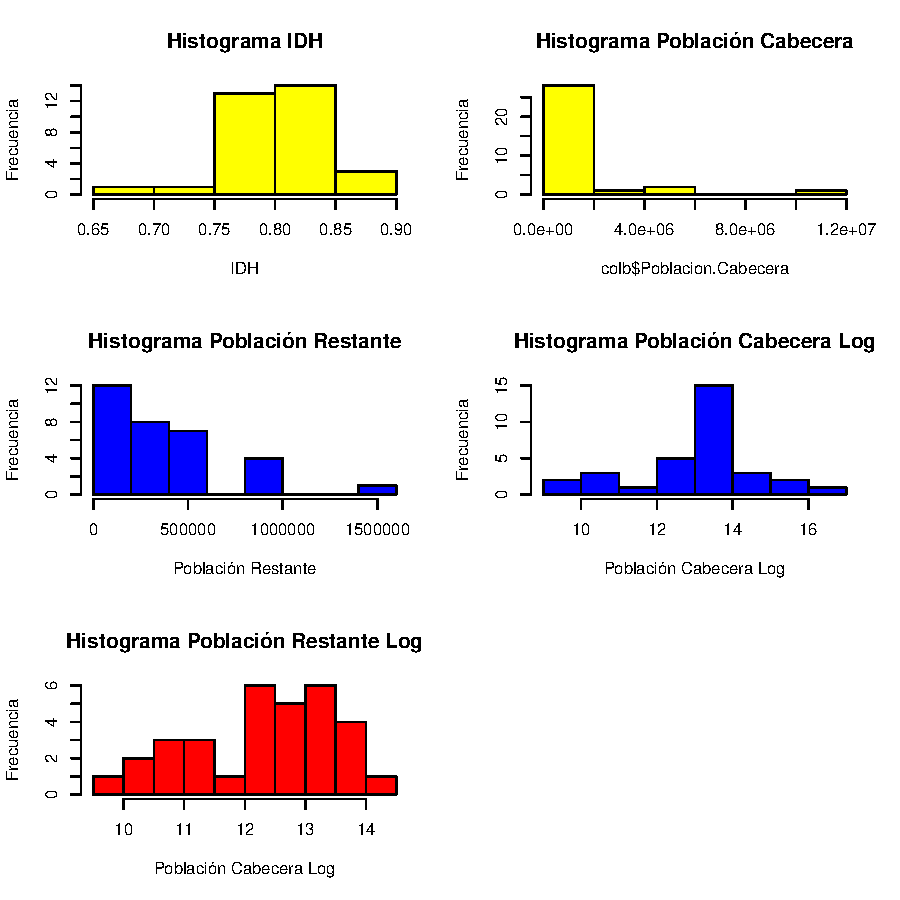
\includegraphics{proyectoLatex-barplots}
\caption{Distribución de Indicadores}

\end{figure}

\clearpage

\section{Exploración Bivariada}

Para la sección se explorará la relación a nivel de correlación entre el IDH y las demás variables, las cuales están ligadas a la población.

% Table created by stargazer v.5.2.2 by Marek Hlavac, Harvard University. E-mail: hlavac at fas.harvard.edu
% Date and time: vie., jun. 29, 2018 - 7:23:04 p. m.
\begin{table}[!htbp] \centering 
  \caption{Correlación IDH y demás variables} 
  \label{corrDem} 
\begin{tabular}{@{\extracolsep{5pt}} cc} 
\\[-1.8ex]\hline 
\hline \\[-1.8ex] 
cabeLog & restoLog \\ 
\hline \\[-1.8ex] 
$0.487$ & $0.177$ \\ 
\hline \\[-1.8ex] 
\end{tabular} 
\end{table} 
Ahora observemos la correlación entre variables independientes
  
% Table created by stargazer v.5.2.2 by Marek Hlavac, Harvard University. E-mail: hlavac at fas.harvard.edu
% Date and time: vie., jun. 29, 2018 - 7:23:04 p. m.
\begin{table}[!htbp] \centering 
  \caption{Correlación entre variables independientes} 
  \label{corrTableX} 
\begin{tabular}{@{\extracolsep{5pt}} ccc} 
\\[-1.8ex]\hline 
\hline \\[-1.8ex] 
 & cabeLog & restoLog \\ 
\hline \\[-1.8ex] 
cabeLog & 1 &  \\ 
restoLog & 0.84 & 1 \\ 
\hline \\[-1.8ex] 
\end{tabular} 
\end{table}  
Lo visto en la Tabla \ref{corrTableX} se refuerza claramente en la Figura \ref{corrPlotX}.

\begin{figure}[h]
\centering
\begin{adjustbox}{width=7cm,height=7cm,clip,trim=1.5cm 0.5cm 0cm 1.5cm}

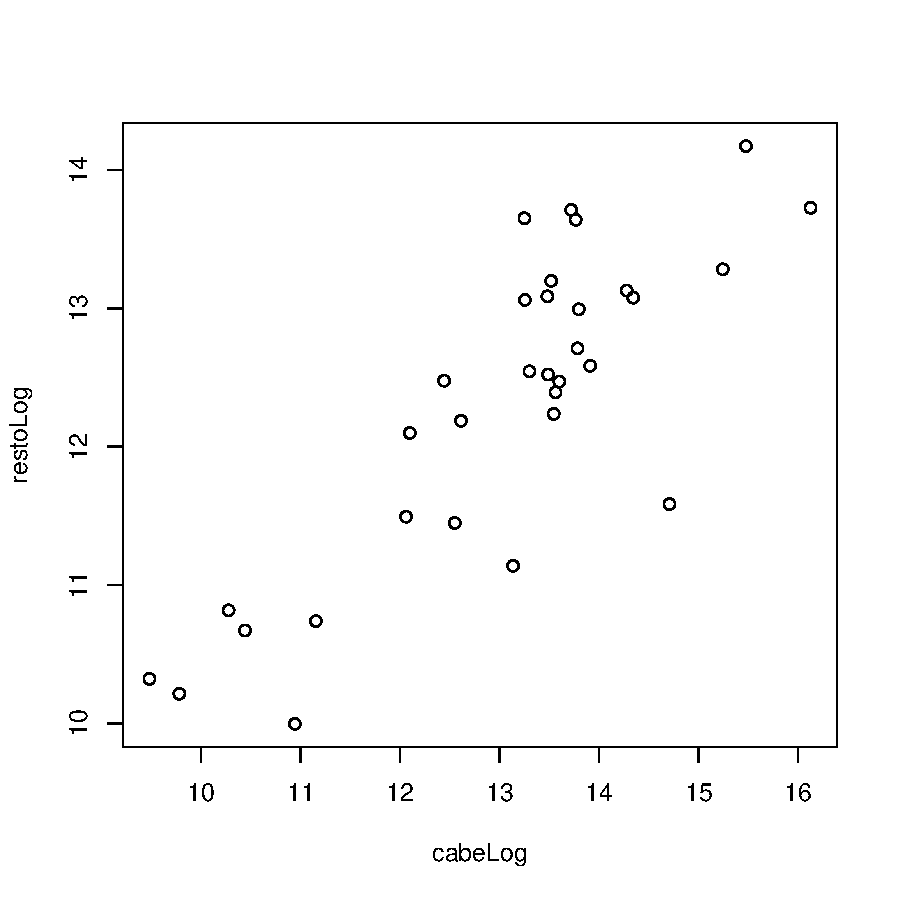
\includegraphics{proyectoLatex-corrPlotX}

\end{adjustbox}
\caption{correlación entre predictores}
\label{corrPlotX}
\end{figure}

\clearpage

\section{Modelos de Regresión}

Finalmente, vemos los modelos propuestos. Primero sin la población resto como independiente, y luego con está. Los resultados se muestran en la Tabla \ref{regresiones} de la página \pageref{regresiones}.


% Table created by stargazer v.5.2.2 by Marek Hlavac, Harvard University. E-mail: hlavac at fas.harvard.edu
% Date and time: vie., jun. 29, 2018 - 7:23:04 p. m.
\begin{table}[!htbp] \centering 
  \caption{Modelos de Regresión} 
  \label{regresiones} 
\begin{tabular}{@{\extracolsep{5pt}}lcc} 
\\[-1.8ex]\hline 
\hline \\[-1.8ex] 
 & \multicolumn{2}{c}{\textit{Dependent variable:}} \\ 
\cline{2-3} 
\\[-1.8ex] & \multicolumn{2}{c}{IDH} \\ 
\\[-1.8ex] & (1) & (2)\\ 
\hline \\[-1.8ex] 
 cabeLog & 0.013$^{***}$ & 0.031$^{***}$ \\ 
  & (0.004) & (0.007) \\ 
  & & \\ 
 restoLog &  & $-$0.030$^{***}$ \\ 
  &  & (0.010) \\ 
  & & \\ 
 Constant & 0.634$^{***}$ & 0.766$^{***}$ \\ 
  & (0.055) & (0.065) \\ 
  & & \\ 
\hline \\[-1.8ex] 
Observations & 32 & 32 \\ 
R$^{2}$ & 0.238 & 0.425 \\ 
Adjusted R$^{2}$ & 0.212 & 0.385 \\ 
Residual Std. Error & 0.037 (df = 30) & 0.033 (df = 29) \\ 
F Statistic & 9.347$^{***}$ (df = 1; 30) & 10.706$^{***}$ (df = 2; 29) \\ 
\hline 
\hline \\[-1.8ex] 
\textit{Note:}  & \multicolumn{2}{r}{$^{*}$p$<$0.1; $^{**}$p$<$0.05; $^{***}$p$<$0.01} \\ 
\end{tabular} 
\end{table} 
Como se vió en la Tabla \ref{regresiones}, cuando está o no presente el \emph{IDH} las variables no pierden significancia.

\clearpage

\section{Exploración Espacial}



Así, propongo que calculemos conglomerados de departamentos usando toda la información de tres de los indicadores. Como nuestras variables son ordinales utilizaremos un proceso de conglomeración donde las distancia serán calculadas usando técnica de k-means de {\bf Mc Queen} propuestas en \cite{macqueen_methods_nodate}. Los tres conglomerados se muestran en la Figura \ref{clustmap}.







\begin{figure}[h]
\centering
%\begin{adjustbox}{width=15cm,height=8cm,clip,trim=1cm 2.5cm 0cm 2.5cm}

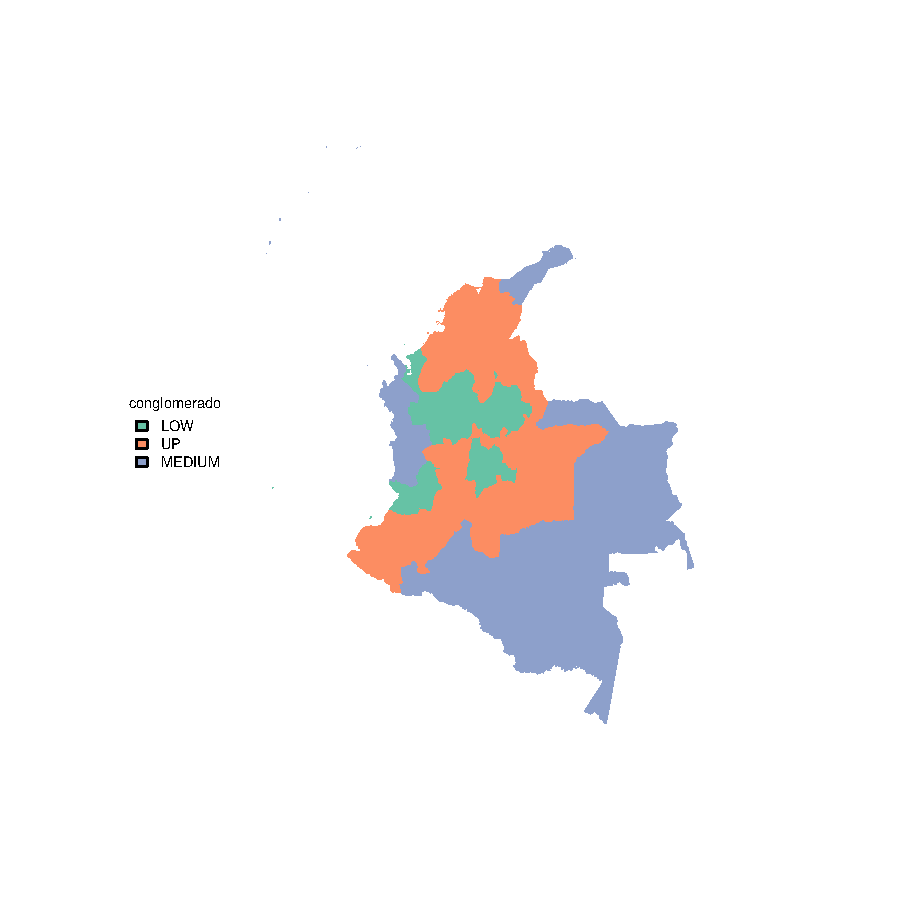
\includegraphics{proyectoLatex-plotMap1}
%\end{adjustbox}
\caption{Departamentos Conglomerados y su IDH}\label{clustmap}
\end{figure}

\bibliographystyle{abbrv}
\renewcommand{\refname}{Bibliografia}
\bibliography{bibliografia}

\end{document}
